\documentclass[10pt,twocolumn,letterpaper]{article}

\usepackage{cvpr}
\usepackage{times}
\usepackage{epsfig}
\usepackage{graphicx, color, xcolor}
\usepackage{amsmath}
\usepackage{amssymb}
\usepackage{bm}
\usepackage[utf8]{inputenc}
\usepackage{fancyhdr}
\usepackage{graphicx}
\usepackage[brazil]{babel}
\usepackage{lipsum}
\usepackage{float}
\setlength{\headheight}{1.5cm}

\fancypagestyle{plain}
\lhead{
\includegraphics[width=5cm,height=2cm]{logoFT.png}}
\rhead{
\includegraphics[width=5cm,height=2cm]{logoUnB.png}}

\renewcommand{\headrulewidth}{1pt}%
}

% Changing the caption and 'References' names to Portuguese.
\addto\captionsenglish{
  \renewcommand{\figurename}{Figura}
  \renewcommand{\tablename}{Tabela}
  \renewcommand{\refname}{Referências bibliográficas}
}

% to-do: Using fontenc with T1 font encoding allows \hyphenation to take words with accents
% as arguments. However, fontenc with T1 mess up with words containing 'ã' in all \subsection{}
% commands.
% If someone knows how to fix it, tell me!
%
%\usepackage[T1]{fontenc}

% Put the words not correctly hyphenated down here. Words with accents must
% be manually hyphenated in the text itself using the '\-' separator. See the examples
% throughout this template.
\hyphenation{co-e-ren-te u-sa-do de-li-mi-ta-do-res a-cer-ca va-lo-res cor-res-pon-den-te re-fe-ren-ci-a-das co-lu-na co-lu-nas em-bo-ra u-ti-li-da-de pro-ce-di-men-to ex-pe-ri-men-to fi-gu-ras}

% If you comment hyperref and then uncomment it, you should delete
% egpaper.aux before re-running latex.  (Or just hit 'q' on the first latex
% run, let it finish, and you should be clear).
\usepackage[breaklinks=true,bookmarks=true]{hyperref}

\cvprfinalcopy % *** Uncomment this line for the final submission

%\def\cvprPaperID{****} % *** Enter the CVPR Paper ID here
%\def\httilde{\mbox{\tt\raisebox{-.5ex}{\symbol{126}}}}

% Pages are numbered in submission mode, and unnumbered in camera-ready
% \ifcvprfinal\pagestyle{empty}\fi
%\setcounter{page}{1}


\begin{document}
%%%%%%%%% TITLE
\title{Experimento 2: Imperfeições AC dos Amplificadores Operacionais}

\author{Aluno 1\\
% To save space, use either the email address or home page, not both
{\tt\small 231012826@aluno.unb.br}\\
% Matrícula do primeiro autor
{\tt\small 231012826}\\
% Turma
{\tt\small Turma T02}
}

\maketitle
%\thispagestyle{empty}

%%%%%%%%% OBJETIVO

\begin{objetivo}
% Resumo com não mais de 250 palavras.
Aqui deve ser o objetivo do relatório.

\end{objetivo}

%%%%%%%%% BODY TEXT
\section{Introdução}
Aqui deve ser apresentada uma pequena introdução de cada um dos assuntos abordados pelo roteiro.

%------------------------------------------------------------------------
\section{Fundamentação teórica}

A {\em Fundamentação teórica} deve apresentar a teoria necessária para a compreensão, execução e análise do experimento. Nesta seção têm de ser incluídas todas as equações pertinentes, entretanto, não convém que valores numéricos sejam introduzidos. Os valores específicos de resistência elétrica, capacitância, indutância, etc., utilizados em la\-bo\-ra\-tó\-rio podem ser apresentados nas seções {\em Procedimento experimental}, {\em Simulações} e {\em Resultados e análises}. 

%-------------------------------------------------------------------------

%-------------------------------------------------------------------------


%-------------------------------------------------------------------------
\newpage
\section{Simulações}

\subsection{Buffer}

Primeiro o circuito é montado com $R_1=\infty$ e $R_2=0$, fazendo da configuração não inversora um circuito Buffer (ou seguidor de tensão).

A saída deve ter amplitude de 1.26V, mas como o ganho é unitário, a entrada também deve ter amplitude de 1.26V.

\begin{figure}[h]
\caption{Circuito não inversor (buffer)}
\begin{center}
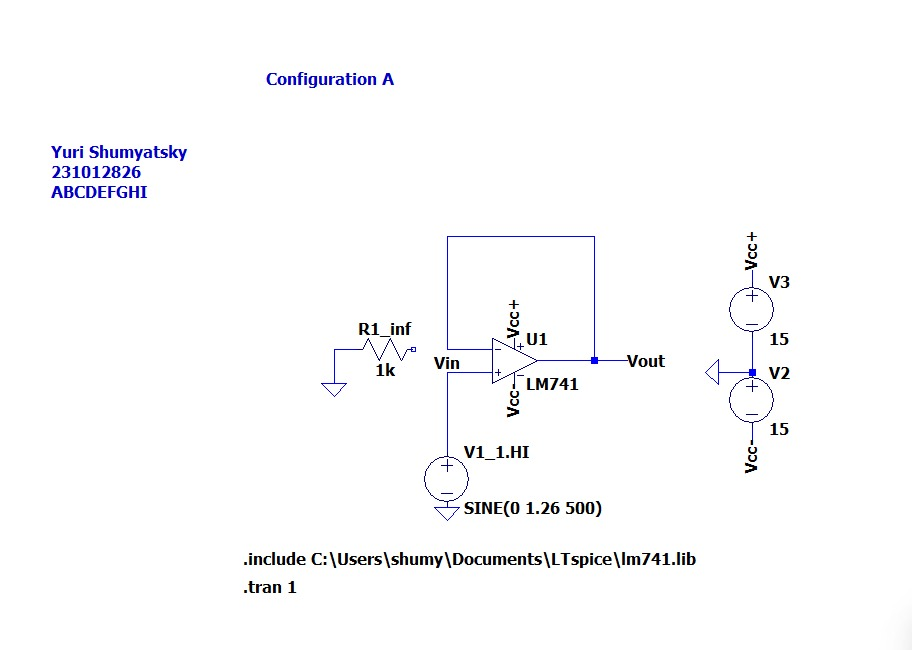
\includegraphics[scale=0.25]{figuras/fig1}
\end{center}
\end{figure}

Segue o plot das tensões de entrada e saída.

\begin{figure}[h]
\caption{Entrada e saída circuito buffer}
\begin{center}
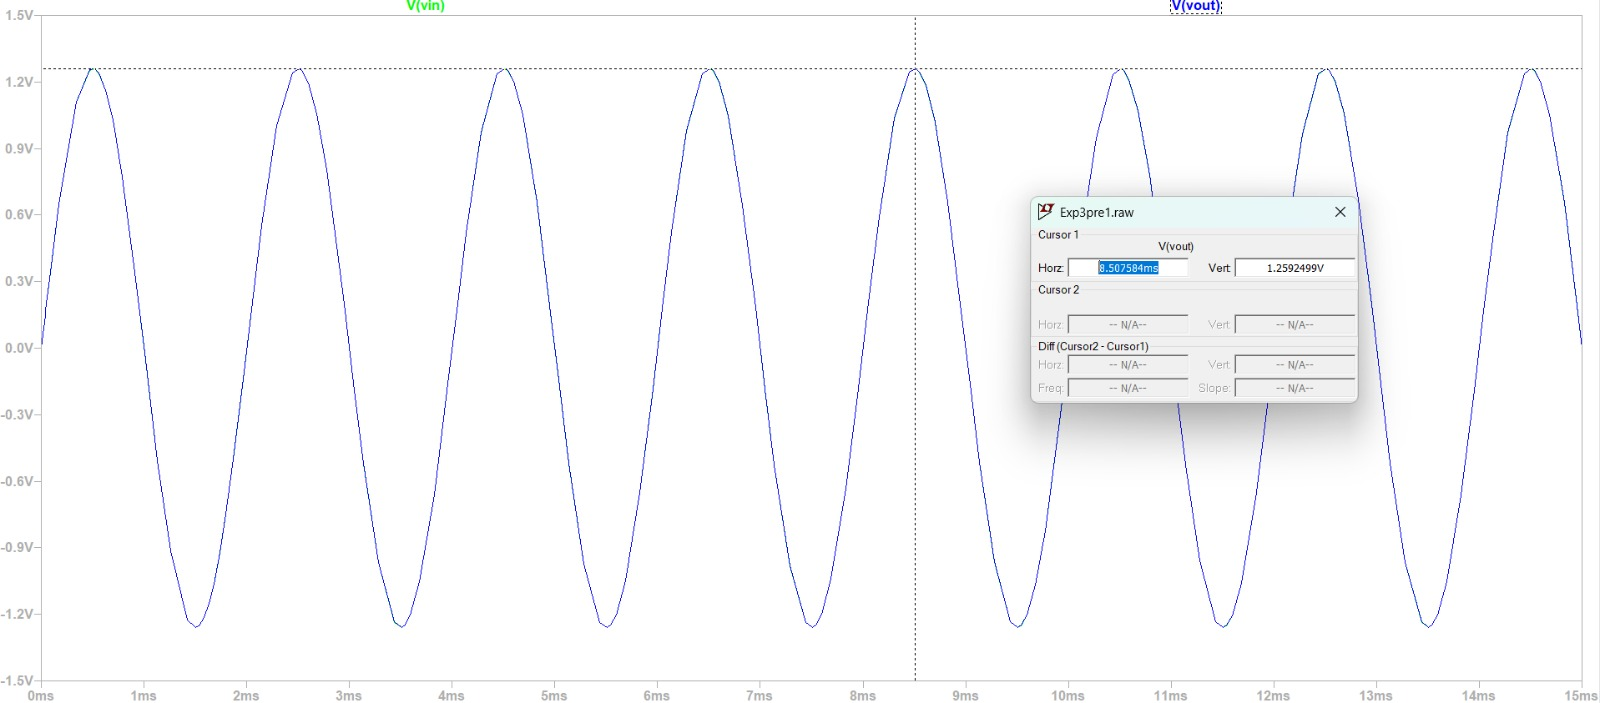
\includegraphics[scale=0.15]{figuras/fig2}
\end{center}
\end{figure}

Para encontrar a frequência de corte, foi utilizada uma análise AC para encontrar a frequência em que a amplitude cai para $(0.71)(1.26V)$.	Isso é feito ao verificar que deve ser subtraído  $20log(\sqrt{2})$ da amplitude em dB, o que equivale a subtrair 3dB pois a tensão é constante.

\begin{figure}[h]
\caption{Análise da frequência de corte}
\begin{center}
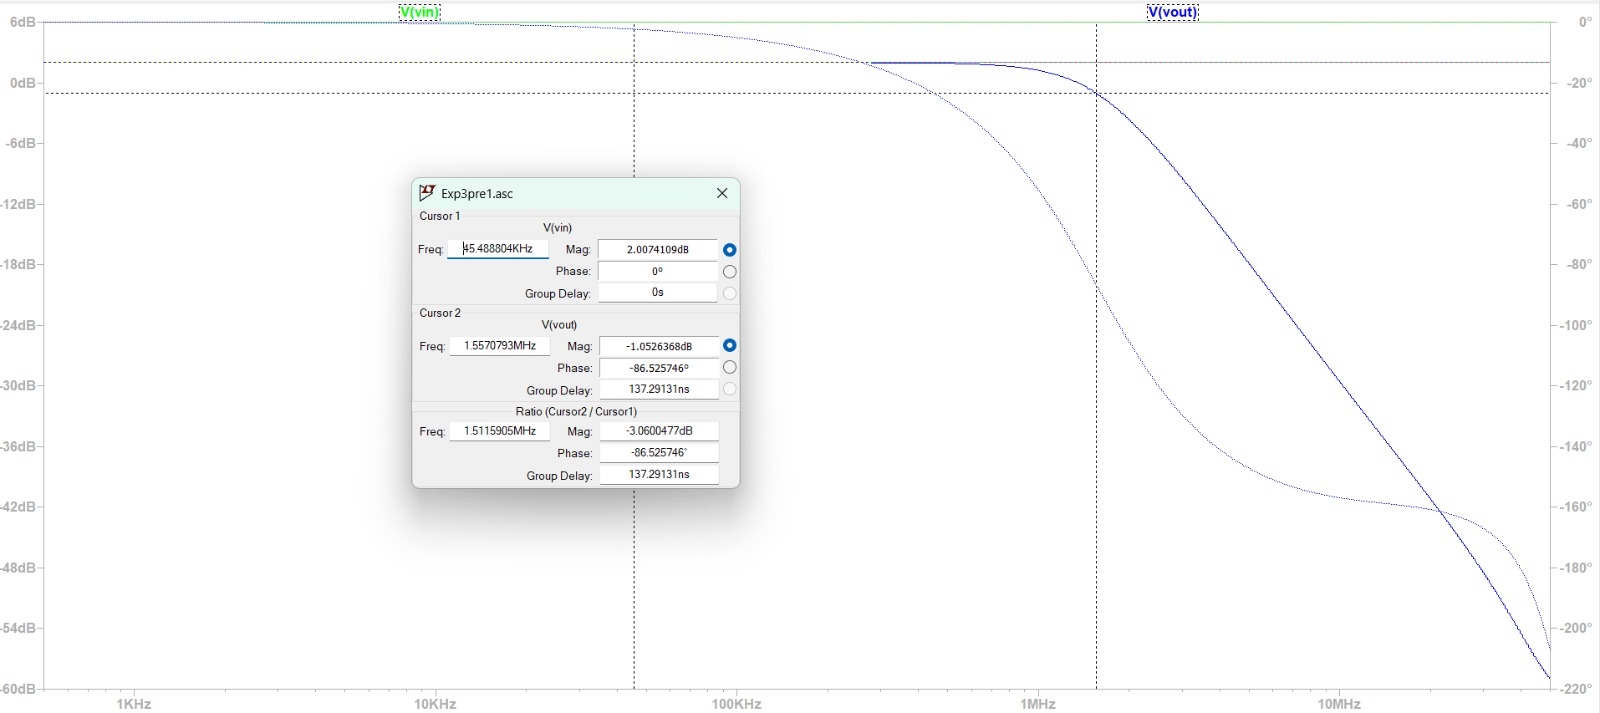
\includegraphics[scale=0.15]{figuras/fig3}
\end{center}
\end{figure}

Como pode ser observado, a $f_c$ encontrada é de 1.557MHz.

Em seguida, é plotado o ganho do circuito em seu bode plot.

\begin{figure}[h]
\caption{Plot do ganho do circuito}
\begin{center}
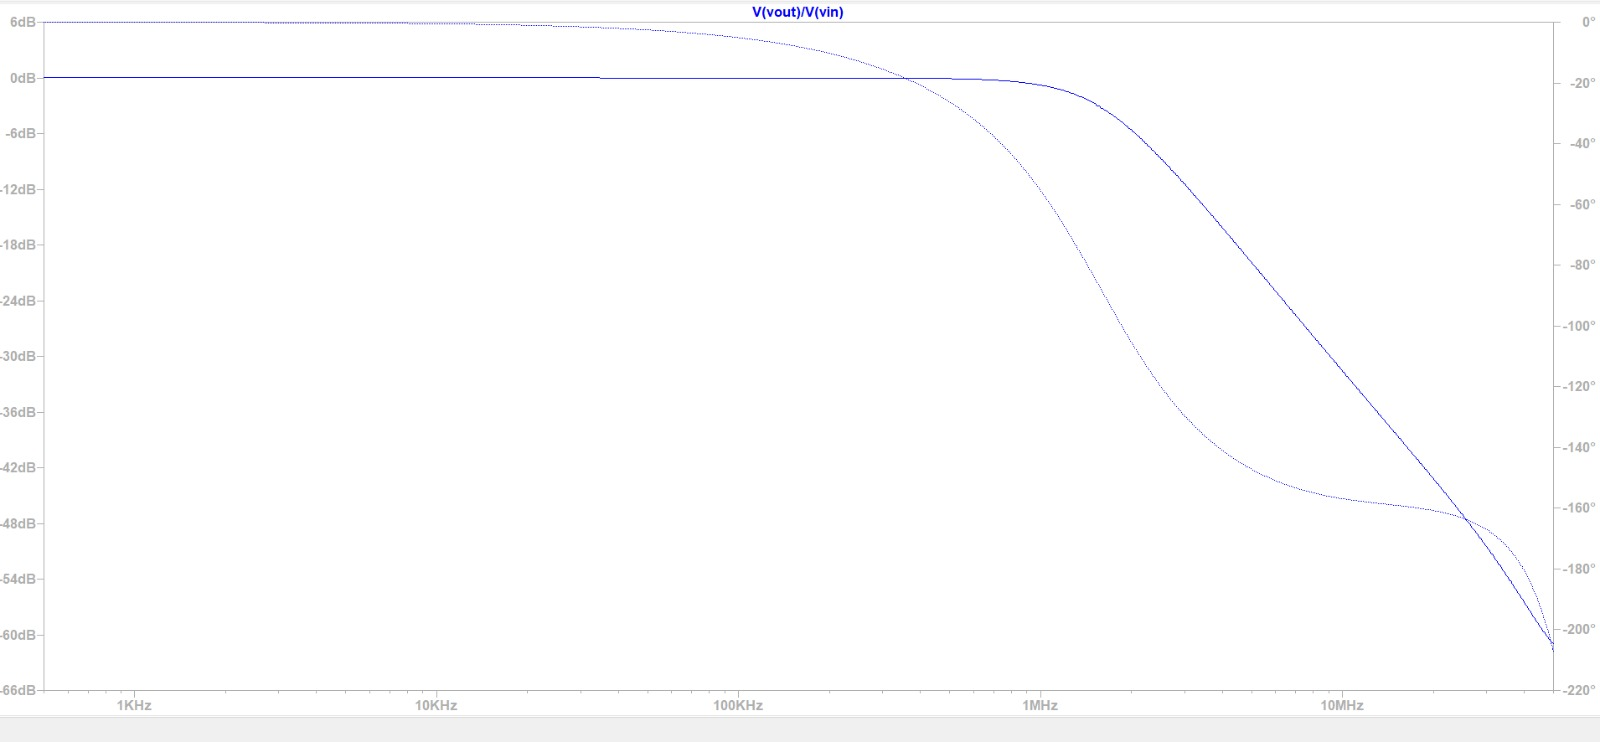
\includegraphics[scale=0.15]{figuras/fig4}
\end{center}
\end{figure}

O produto ganho $\times$ banda passante do ampop nesse circuito é $A\cdot f_c$, sendo $A$ o ganho em frequências baixas (menores que $f_c$). Como nesse circuito $A=1$ e $f_c=1.557MHz$, o produto tem valor de $1.557\cdot10^6$, como pode ser observado no seguinte gráfico.

\begin{figure}[h]
\caption{GBW}
\begin{center}
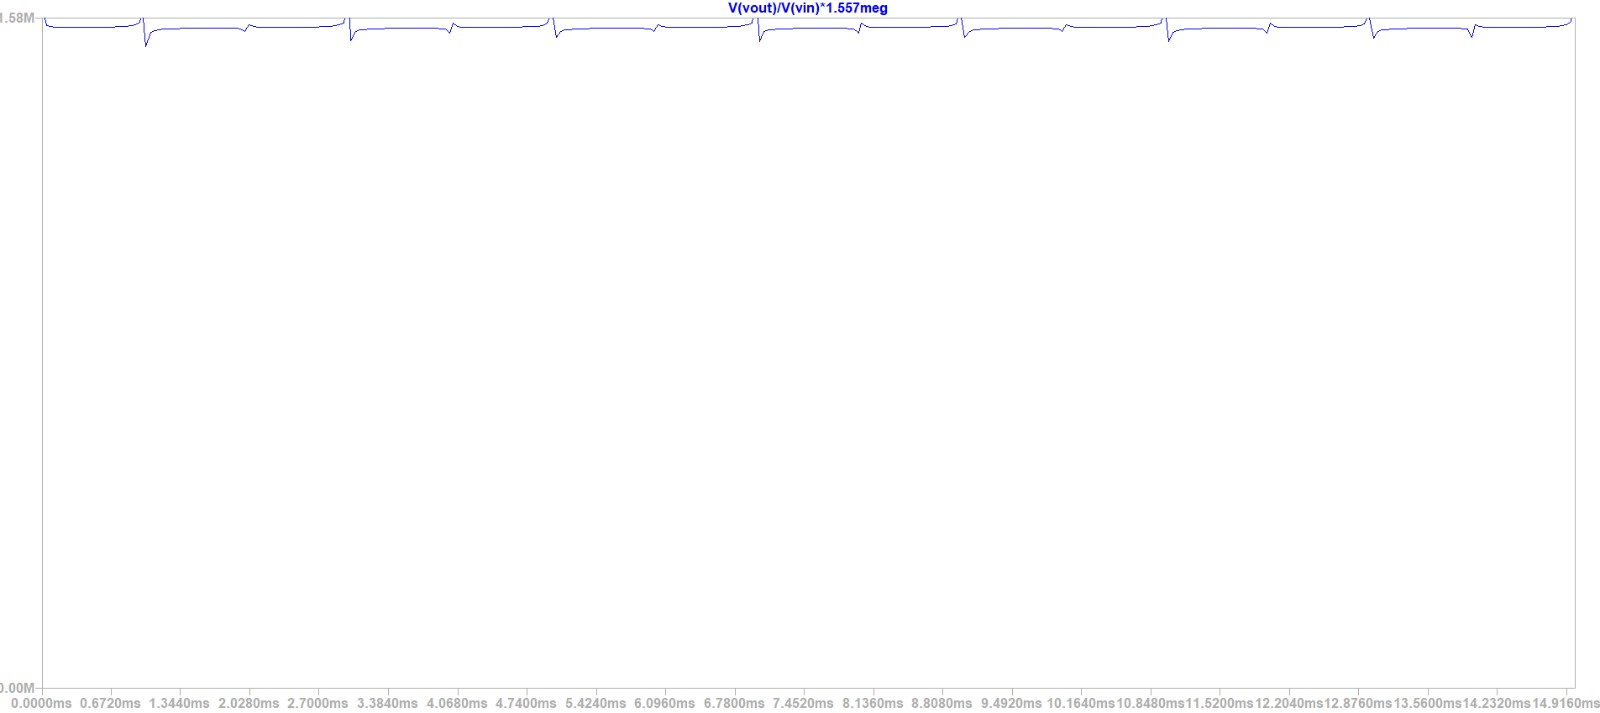
\includegraphics[scale=0.15]{figuras/fig5}
\end{center}
\end{figure}

\newpage
\subsection{Não inversor com ganho baixo}

O circuito agora é montado com $R_1=1k\Omega$ e $R_2=13k\Omega$. O ganho do circuito é 14, então para que a tensão de saída possua amplitude de $1.26V$ a tensão de entrada deve ter amplitude de $0.09V$.

\begin{figure}[h]
\caption{Circuito com ganho baixo}
\begin{center}
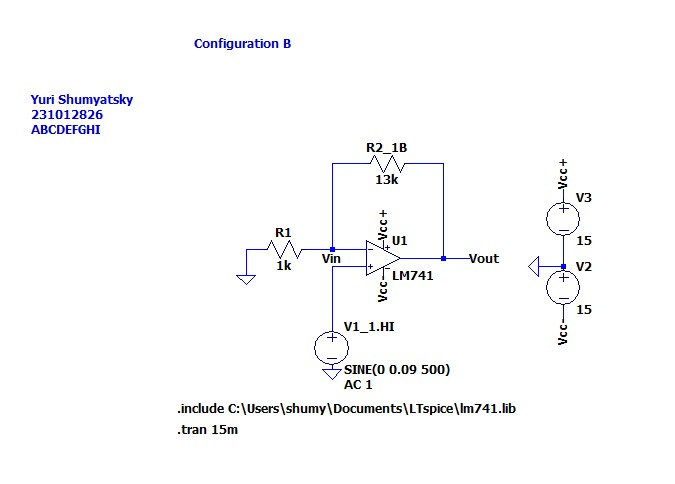
\includegraphics[scale=0.25]{figuras/fig6}
\end{center}
\end{figure}

Seguem as tensões de entrada e saída.

\begin{figure}[h]
\caption{Entrada e saída circuito com ganho baixo}
\begin{center}
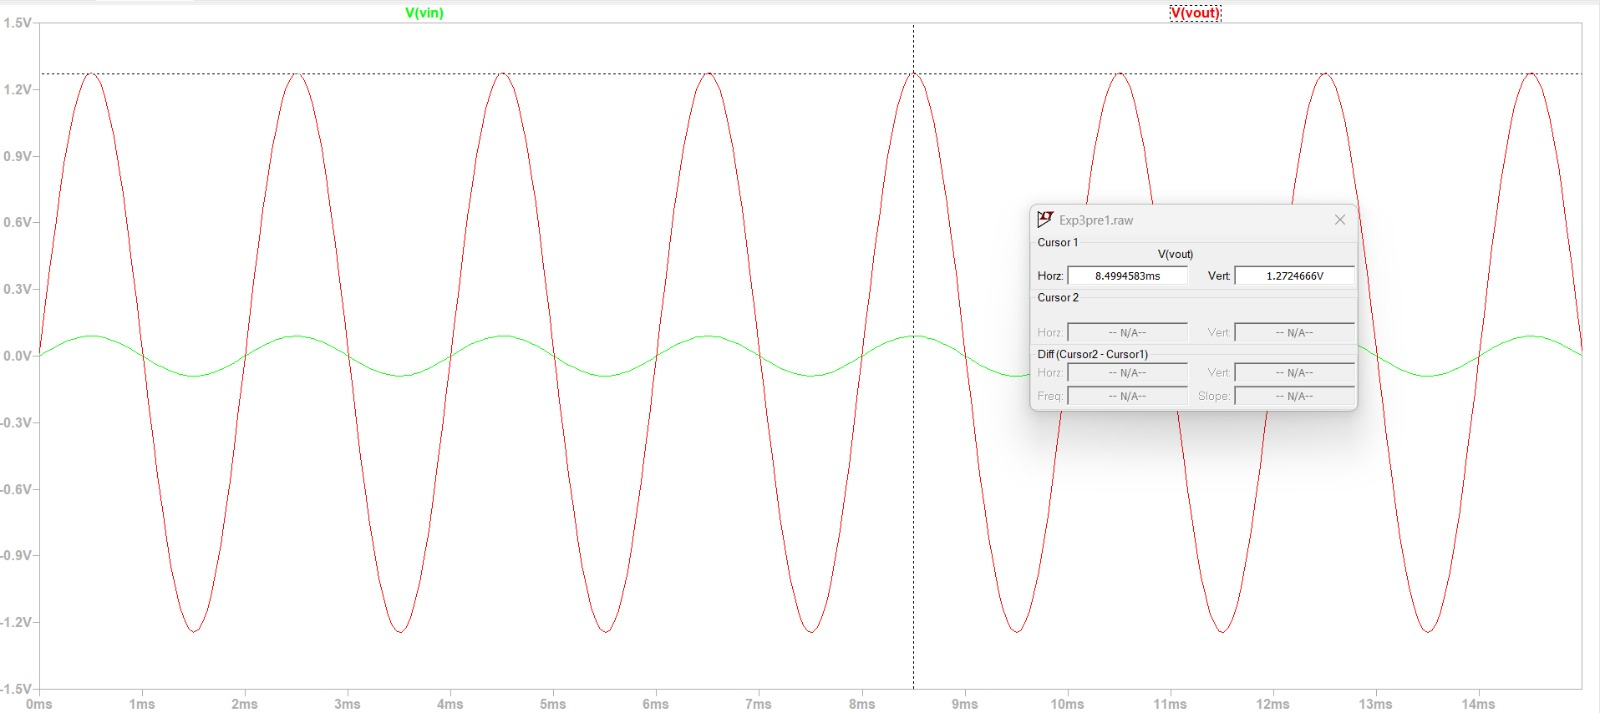
\includegraphics[scale=0.15]{figuras/fig7}
\end{center}
\end{figure}


O procedimento para encontrar a frequência de corte é análogo, tendo como resultado $f_c= 1.285$MHz

\begin{figure}[h]
\caption{Análise frequência de corte (circuito 2)}
\begin{center}
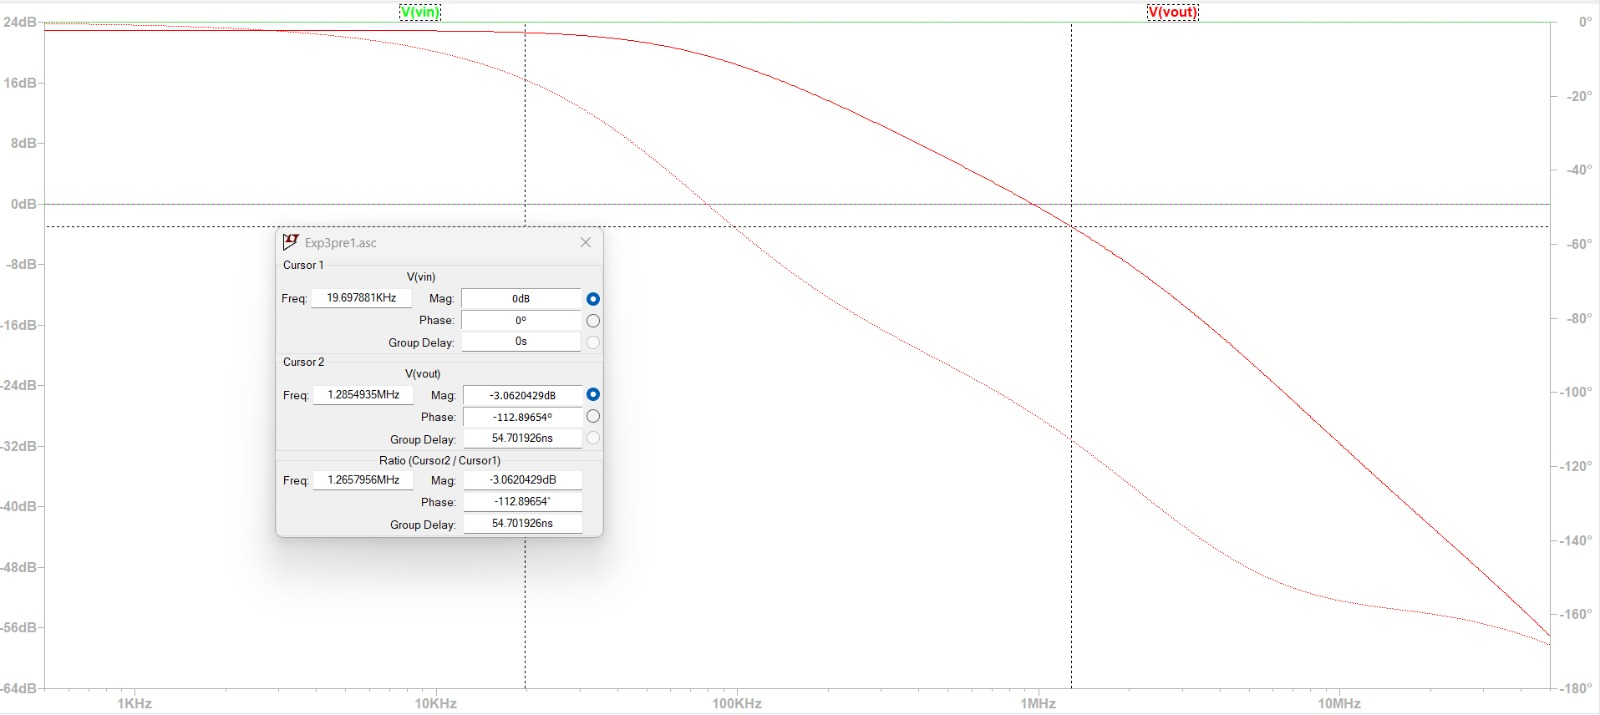
\includegraphics[scale=0.15]{figuras/fig8}
\end{center}
\end{figure}

\newpage
Segue o bode plot do ganho do circuito.

\begin{figure}[h]
\caption{Bode plot ganho (circuito 2)}
\begin{center}
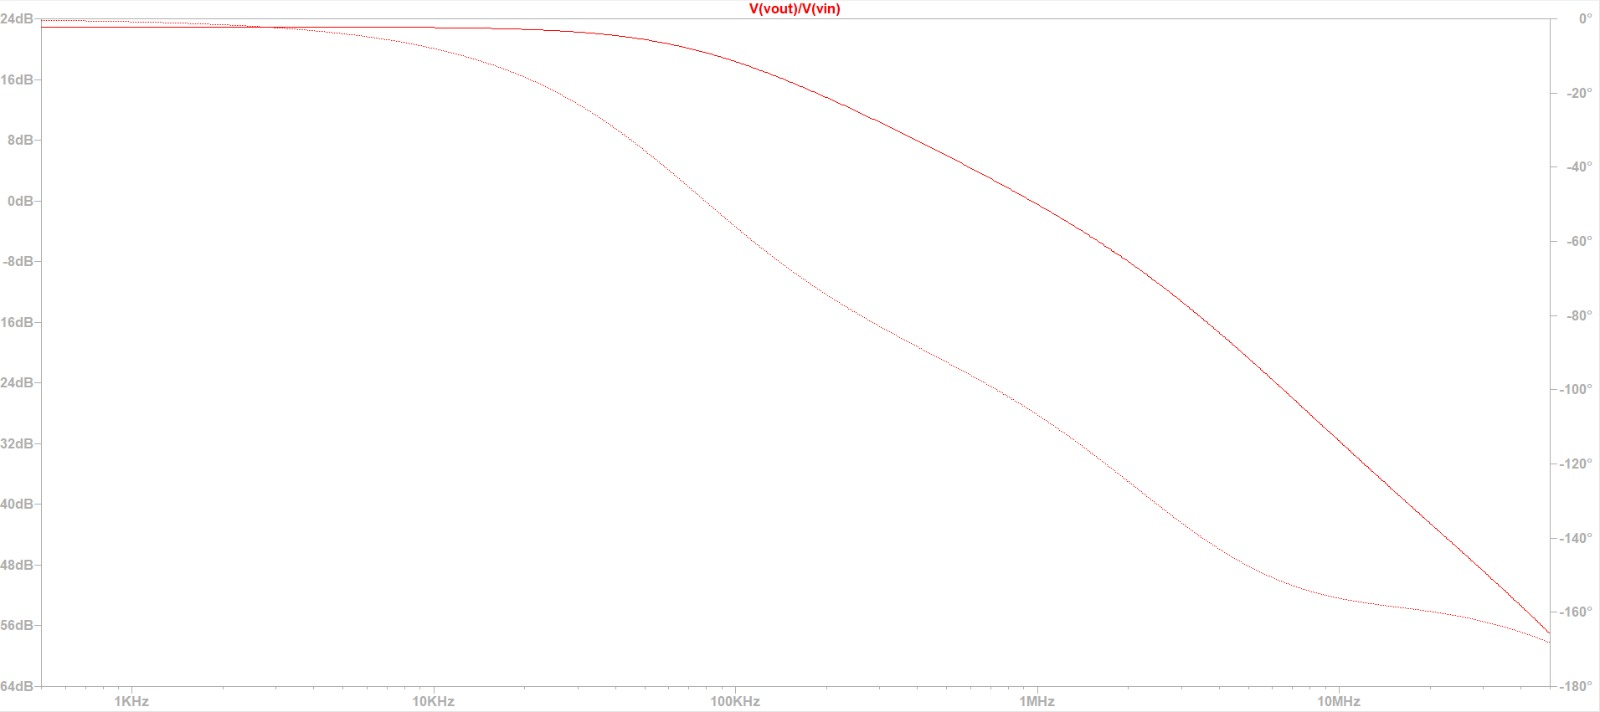
\includegraphics[scale=0.15]{figuras/fig9}
\end{center}
\end{figure}

O produto ganho $\times$ banda passante do ampop nesse circuito é $A\cdot f_c$, sendo portanto $GBW = 14\cdot1.285\cdot10^6=17.99\cdot10^6$

\begin{figure}[h]
\caption{GBW (circuito 2)}
\begin{center}
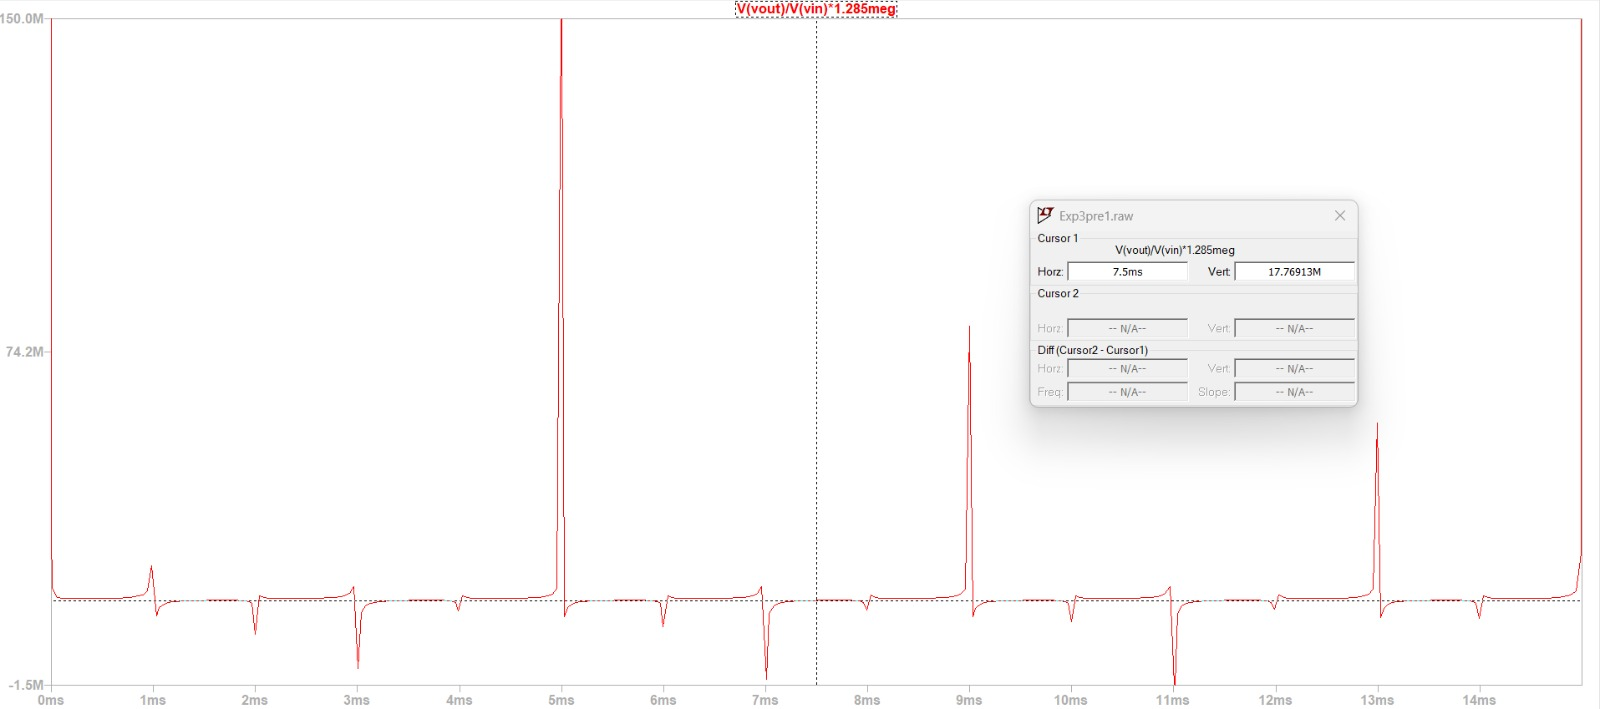
\includegraphics[scale=0.15]{figuras/fig10}
\end{center}
\end{figure}

\subsection{Circuito não inversor de ganho alto}

O circuito agora é remontado com $R_1=1k\Omega$ e $R_2=101k\Omega$. Assim, o ganho é de 102, o que faz com que para que a saída possua amplitude de $1.26V$, a entrada deve ter $0.012V$.

\begin{figure}[h]
\caption{Circuito 3}
\begin{center}
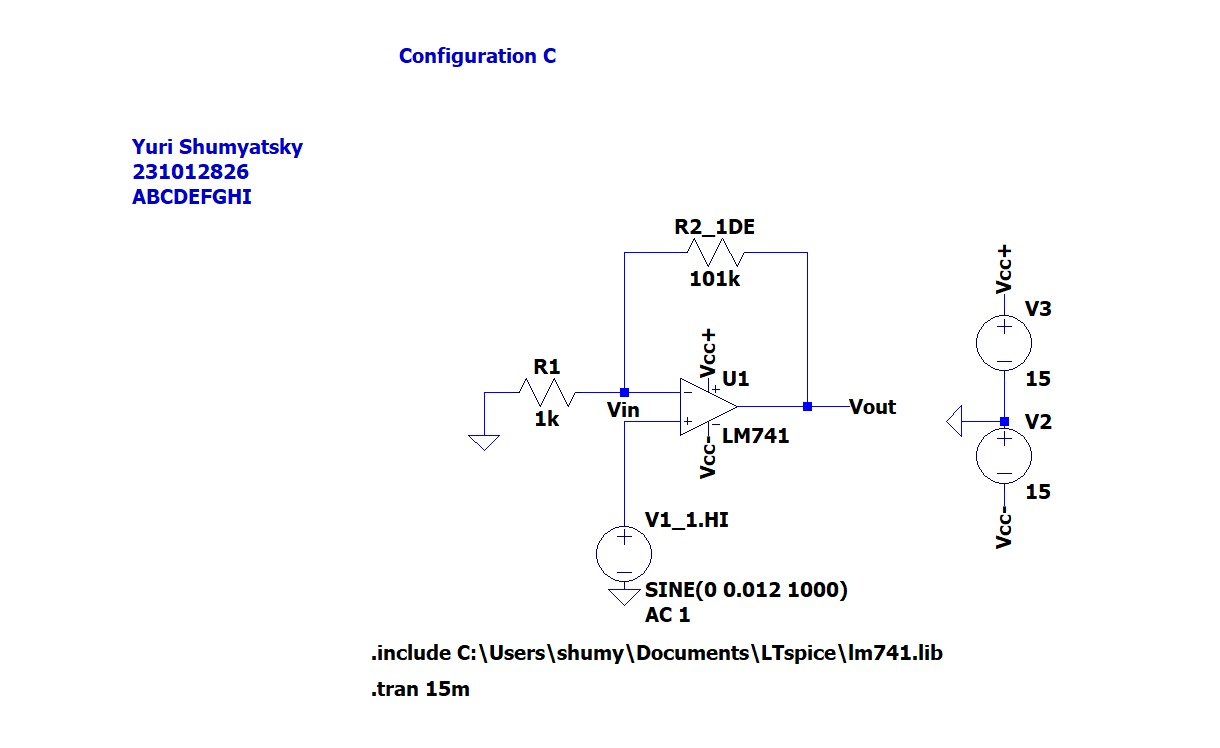
\includegraphics[scale=0.2]{figuras/fig11}
\end{center}
\end{figure}

Seguem a entrada e saída plotadas.

\begin{figure}[h]
\caption{Tensões de entrada e saída (circuito 3)}
\begin{center}
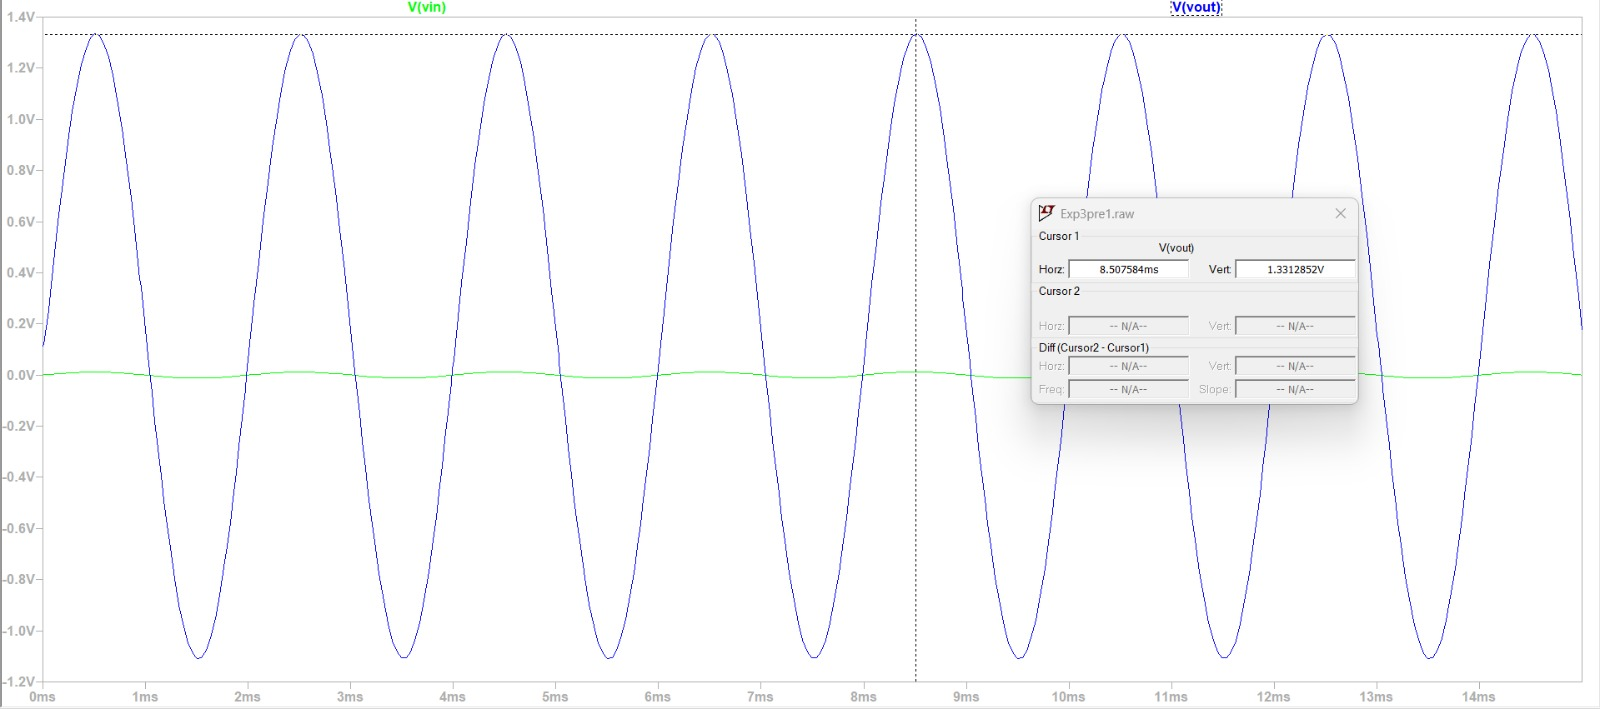
\includegraphics[scale=0.15]{figuras/fig12}
\end{center}
\end{figure}

Encontrar a frequência de corte novamente é análogo, resultando em $f_c=1.269$MHz.

\begin{figure}[h]
\caption{Análise frequência de corte (circuito 3)}
\begin{center}
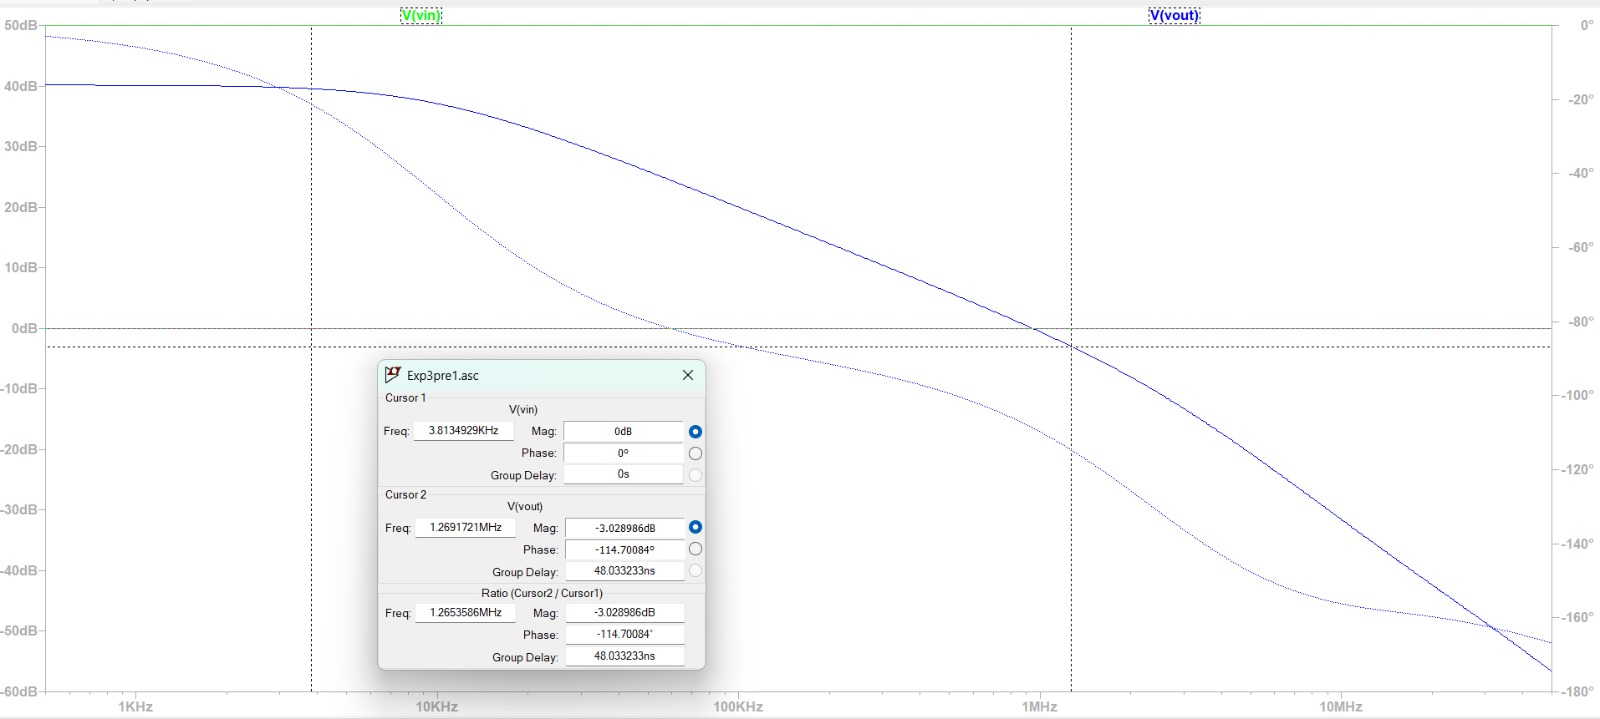
\includegraphics[scale=0.15]{figuras/fig13}
\end{center}
\end{figure}

A figura 14 é o bode plot do ganho do circuito.

\begin{figure}[h]
\caption{Bode plot do ganho (circuito 3)}
\begin{center}
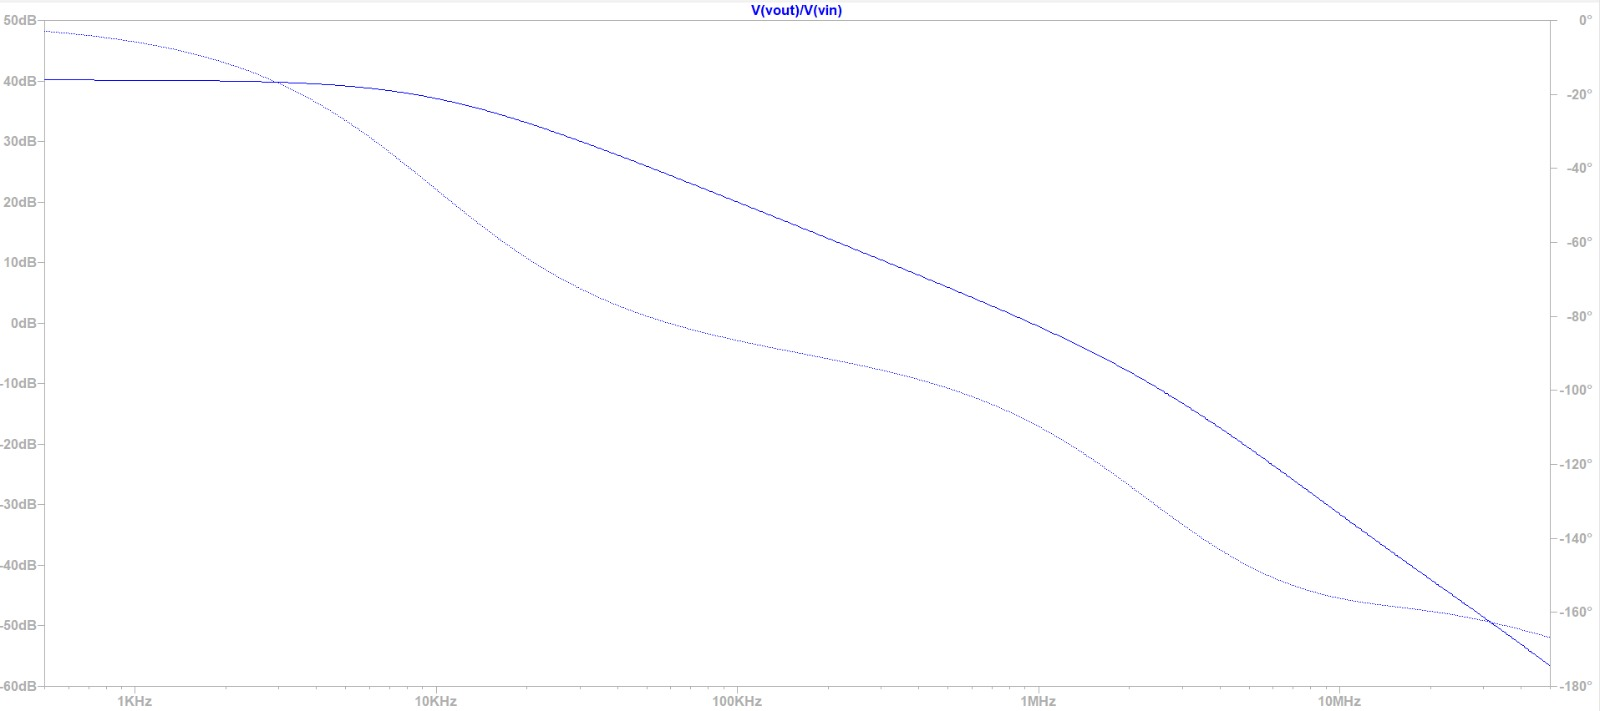
\includegraphics[scale=0.15]{figuras/fig14}
\end{center}
\end{figure}

\newpage
O produto ganho $\times$ banda passante do ampop nesse circuito continua sendo $A\cdot f_c$, sendo portanto $GBW = 102\cdot1.269\cdot10^6=129.4\cdot10^6$ O analisado bate com o razoável, porém com certa margem de erro. 

\begin{figure}[h]
\caption{GBW (circuito 3)}
\begin{center}
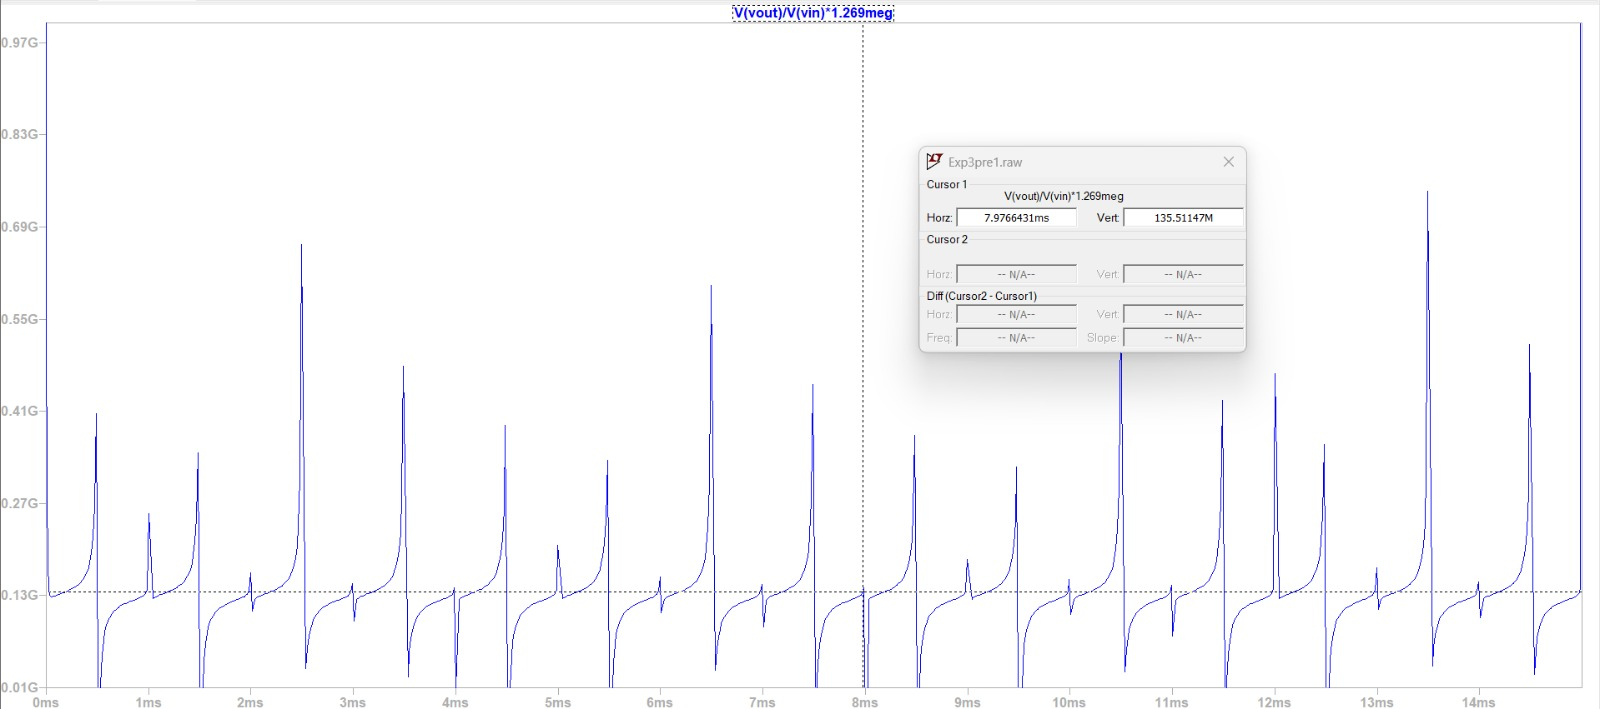
\includegraphics[scale=0.15]{figuras/fig15}
\end{center}
\end{figure}

%-------------------------------------------------------------------------


{\small
\bibliography{egbib}
\bibliographystyle{ieee_fullname}
}

\end{document}
